\subsection{Reinforcement learning} \label{sec:rl}

One of the original motivations for developing the model structures in  \verb|RobustNeuralNetworks.jl| was to guarantee stability and robustness in learning-based control. Recently, we have shown that with a controller architecture based on a nonlinear version of classical Youla-Kucera parameterization \cite{Youla++1976}, one can learn over a space of stabilizing controllers for linear and nonlinear systems using standard reinforcement learning techniques, so long as the control policy is parameterized by a contracting, Lipschitz-bounded REN  \cite{Wang+Manchester2022,Wang++2022,Barbara++2023}. This is an exciting result for learning-based controllers in safety-critical systems, such as in robotics.

In this example, we will demonstrate how to train an LBDN controller with \textit{reinforcement learning} (RL) for a simple nonlinear dynamical system. This controller will not have any stability guarantees. The purpose of this example is simply to showcase the steps required to set up RL experiments for more complex systems with RENs and LBDNs.

% Overview
\subsubsection{Overview} \label{sec:rl-overview}

Consider the simple mechanical system shown in Figure \ref{fig:rl-box}: a box of mass $m$ sits in a tub of fluid, held between the walls by two springs each with spring constant $k/2.$ The box can be pushed with a force $u.$ Its dynamics are
\begin{equation} \label{eqn:box-dynamics}
m\ddot{q} = u - kq - \mu \dot{q}|\dot{q}|
\end{equation}
where $\mu$ is the viscous damping coefficient due to the box moving through the fluid, and $\dot{q},\ddot{q}$ denote the velocity and acceleration of the box, respectively.

\begin{figure}[!t]
    \centering
    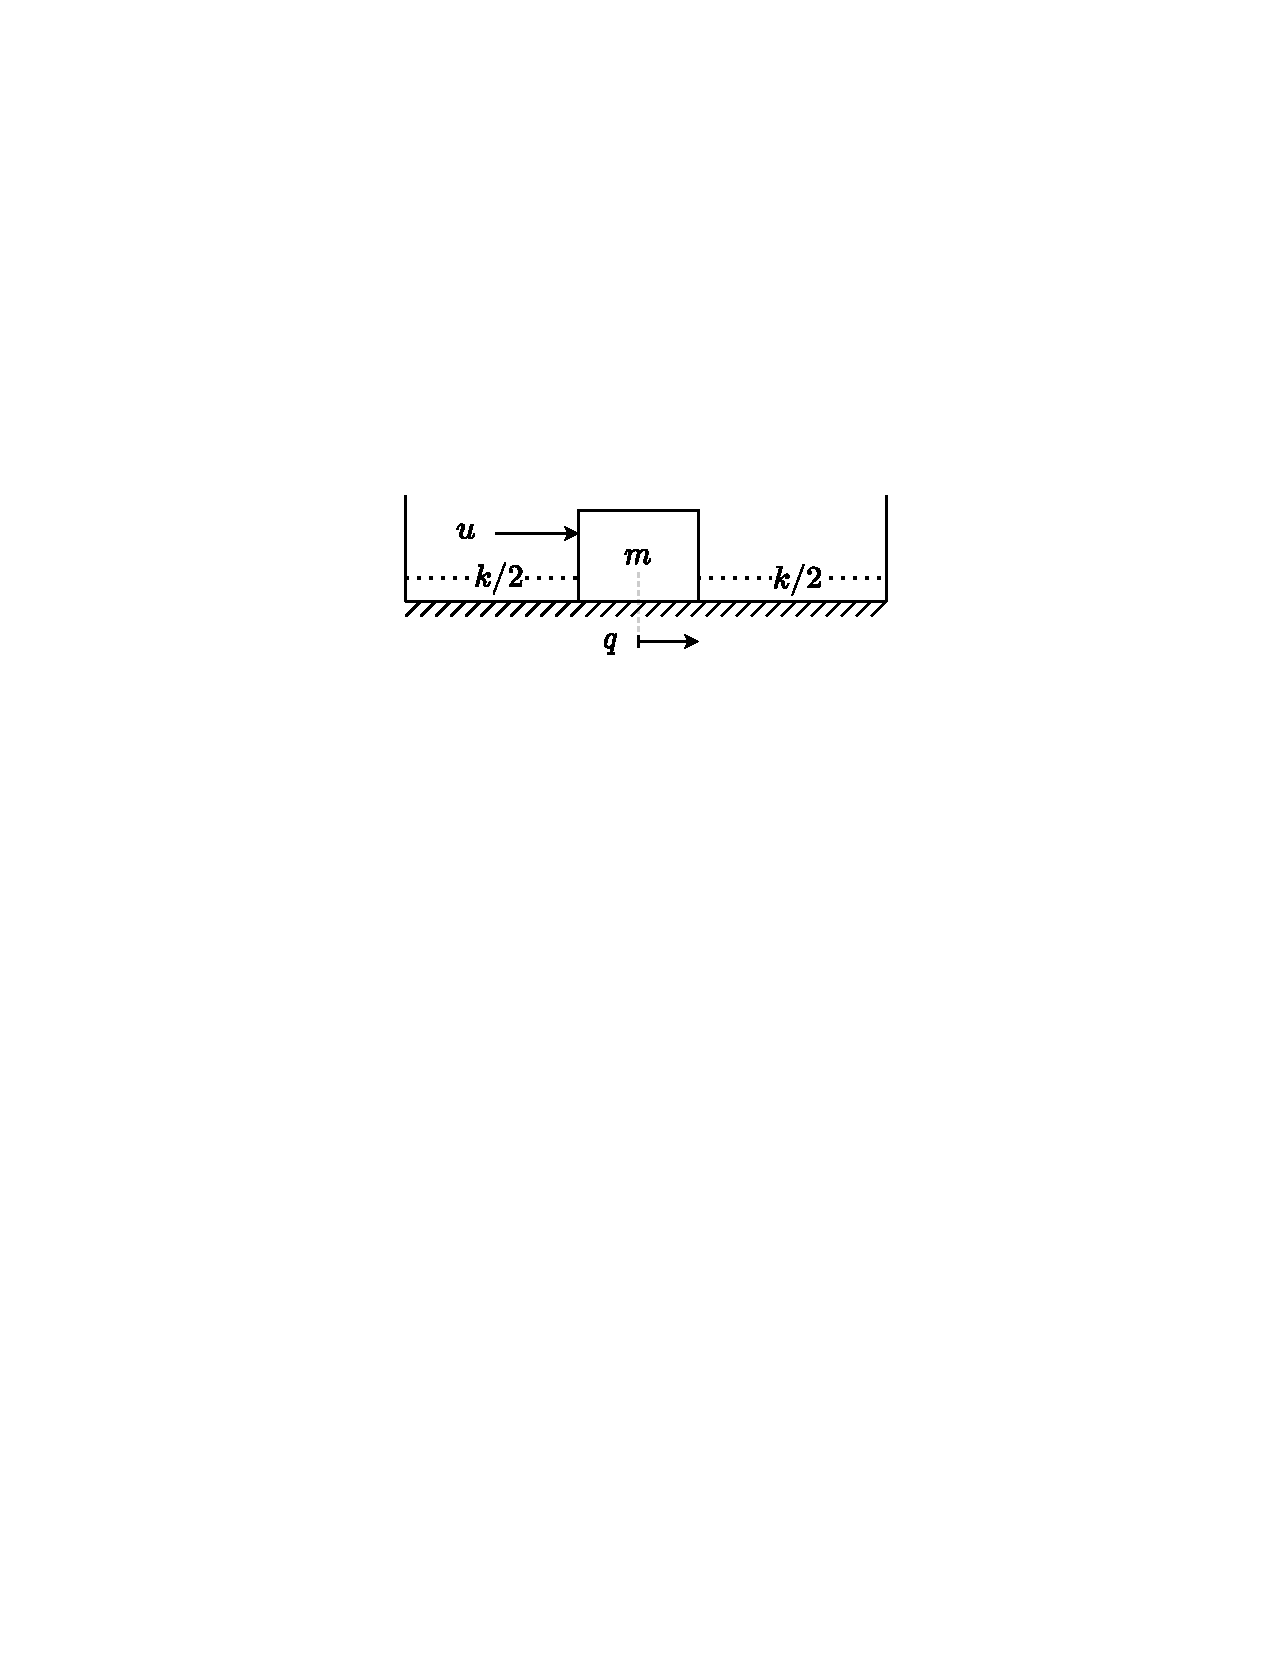
\includegraphics[width=0.27\textwidth]{Images/mass_rl.pdf}
    \caption{Mechanical system to be controlled. A box sits in a tub of fluid, suspended between two springs, and can be pushed by a force $u$ to different horizontal positions $q$.}
    \label{fig:rl-box}
\end{figure}

We can write this as a (nonlinear) state-space model with state $x = (q,\dot{q})^\top,$ control input $u,$ and dynamics
\begin{equation}
\dot{x} = f(x,u) := \begin{bmatrix}
\dot{q} \\ (u - kq - \mu \dot{q}|\dot{q}|)/m
\end{bmatrix}.
\end{equation}
This is a continuous-time model of the dynamics. For our purposes, we need a discrete-time model. We can discretize the dynamics using a forward Euler approximation to get
\begin{equation}
x_{t+1} = f_d(x_t,u_t) := x_t + \Delta t \cdot f(x_t, u_t)
\end{equation}
where $\Delta t$ is the time-step. This approximation typically requires a small time-step for numerical stability, but is sufficient for our simple example. If physical accuracy was of concern, one could use a fourth (or higher) order Runge-Kutta scheme.

Our aim is to learn a controller $u = \mathcal{K}_\theta(x, q_\mathrm{ref}),$ defined by some learnable parameters $\theta,$ that can push the box to any goal position $q_\mathrm{ref}$ that we choose. Specifically, we want the box to:
\begin{enumerate}
    \item reach a (stationary) goal position $q_\mathrm{ref}$
    \item within a time period $T$.
\end{enumerate}
The force required to keep the box at a static equilibrium position $q_\mathrm{ref}$ is $u_\mathrm{ref} = k q_\mathrm{ref}$ from Equation \ref{eqn:box-dynamics}. We can encode these objectives into a cost function $J_\theta$ and write our RL problem as
\begin{equation} \label{eqn:rl-costfunc}
\min_\theta \mathbb{E} \left[ J_\theta \right],
\quad
J_\theta = \sum_{t=0}^{T-1} c_1 (\Delta q_t)^2 + c_2 \dot{q}_t^2 + c_3 (\Delta u_t)^2
\end{equation}
where $\Delta q_t = q_t - q_\mathrm{ref}$, $\Delta u_t = u_t - u_\mathrm{ref}$, $c_1, c_2, c_3$ are cost function weights, and the expectation is over different initial and goal positions of the box.


% Problem setup
\subsubsection{Problem setup} \label{sec:rl-setup}

We start by defining the properties of our system and translating the dynamics into Julia code. For this example, we consider a box of mass $m=1$, spring constants $k=5,$ and a viscous damping coefficient $\mu = 0.5$. We will simulate the system over $T = 4$\,s time horizons with a time-step of $\Delta t = 0.02$\,s.

\begin{lstlisting}[language = Julia]
m = 1                   # Mass (kg)
k = 5                   # Spring constant (N/m)
μ = 0.5                 # Viscous damping (kg/m)
Tmax = 4                # Simulation horizon (s)
dt = 0.02               # Time step (s)
ts = 1:Int(Tmax/dt)     # Array of time indices
\end{lstlisting}

Now we can generate the training data. Suppose the box always starts at rest from the zero position, and the goal position can be anywhere in the range $q_\mathrm{ref} \in [-1,1]$. Our training data consists of a batch of 80 randomly-sampled goal positions and corresponding reference forces $u_\mathrm{ref}$.
\begin{lstlisting}[language = Julia]
nx, nref, batches = 2, 1, 80
x0 = zeros(nx, batches)
qref = 2*rand(nref, batches) .- 1
uref = k*qref
\end{lstlisting}

It is good practice (and faster) to simulate all simulation batches at once, so we define our dynamics functions to operate on batches of states and controls. Each row corresponds to a different state or control, and each column corresponds to a simulation for a particular goal position.

\begin{lstlisting}[language = Julia]
f(x::Matrix,u::Matrix) = [x[2:2,:]; (u[1:1,:] - 
    k*x[1:1,:] - μ*x[2:2,:]*abs.(x[2:2,:]))/m]
fd(x::Matrix,u::Matrix) = x + dt*f(x,u)
\end{lstlisting}

RL problems typically involve simulating the system over some time horizon and collecting rewards or costs at each time step. Control policies are trained using approximations of the cost gradient $\nabla J_\theta$, as it is often difficult (or impossible) to compute the exact gradient due to the complexity of dynamics simulators. We refer the reader to \cite{Sutton+Barto2018} for further details, and \verb|ReinforcementLearning.jl| \cite{Tian++2020} for examples in Julia.

For this simple example, we can back-propagate directly through the dynamics function \verb|fd(x,u)| rather than approximating  $\nabla J_\theta$. The simulator below takes a batch of initial states, goal positions, and a controller \verb|model| whose inputs are $[x; q_\mathrm{ref}]$. It computes trajectories of states and controls $z = \{[x_0;u_0], \ldots, [x_{T-1};u_{T-1}]\}$. To avoid the issue of unsupported array mutation when differentiating we use a \verb|Zygote.Buffer| to iteratively store the outputs \cite{Innes2018b}.

\begin{lstlisting}[language = Julia]
using Zygote: Buffer

function rollout(model, x0, qref)
    z = Buffer([zero([x0;qref])], length(ts))
    x = x0
    for t in ts
        u = model([x;qref])
        z[t] = vcat(x,u)
        x = fd(x,u)
    end
    return copy(z)
end
\end{lstlisting}

After computing these trajectories, we will need a function to evaluate the cost given some weightings $c_1,c_2,c_3$.
\begin{lstlisting}[language = Julia]
using Statistics

weights = [10,1,0.1]
function _cost(z, qref, uref)
    Δz = z .- [qref; zero(qref); uref]
    return mean(sum(weights .* Δz.^2; dims=1))
end
cost(z::AbstractVector, qref, uref) = 
    mean(_cost.(z, (qref,), (uref,)))
\end{lstlisting}

% Define a model
\subsubsection{Define a model} \label{sec:rl-model}

We will train an LBDN controller with a Lipschitz bound of $\gamma = 20$. Its inputs are the state $x_t$ and goal position $q_\mathrm{ref}$, while its outputs are the control force $u_t$. We have chosen a model with two hidden layers each of 32 neurons just as an example. For examples of how Lipschitz bounds can be useful in learning robust controllers, see \cite{Barbara++2023,Russo+Proutiere2021,Song++2023}.

\begin{lstlisting}[language = Julia]
using RobustNeuralNetworks

T  = Float64
γ  = 20                 # Lipschitz bound
nu = nx + nref          # Inputs (x and reference)
ny = 1                  # Outputs (control action)
nh = fill(32, 2)        # Hidden layers
model_ps = DenseLBDNParams{T}(nu, nh, ny, γ)
\end{lstlisting}

% Define a loss function
\subsubsection{Define a loss function} \label{sec:rl-loss}

In constructing a loss function for this problem, we refer to Section \ref{sec:explicit-wrappers}. The \verb|model_ps| contain all information required to define a dense LBDN model. However, \verb|model_ps| is not a model that can be evaluated on data: it is a \textit{model parameterization}, and contains the learnable parameters $\theta$. To train an LBDN given some data, we construct the model within the loss function using the \verb|LBDN| wrapper so that the mapping from direct to explicit parameters is captured during back-propagation. Our loss function therefore includes the following three components.

\begin{lstlisting}[language = Julia]
function loss(model_ps, x0, qref, uref)
    model = LBDN(model_ps)            # Model
    z = rollout(model, x0, qref)      # Simulation
    return cost(z, qref, uref)        # Cost
end
\end{lstlisting}

    

% Train the model
\subsubsection{Train the model} \label{sec:rl-train}

Having set up the RL problem, all that remains is to train the controller. The function below trains a model and keeps track of the training loss \verb|tloss| (cost $J_\theta$) for each simulation in our batch of 80. Training is performed with the \verb|Adam| optimizer over 250 epochs with a learning rate of $10^{-3}$.

\begin{lstlisting}[language = Julia]
using Flux

function train_box_ctrl!(
    model_ps, loss_func; 
    epochs=250, lr=1e-3
)
    costs = Vector{Float64}()
    opt_state = Flux.setup(Adam(lr), model_ps)
    for k in 1:epochs

        tloss, dJ = Flux.withgradient(
            loss_func, model_ps, x0, qref, uref)
        Flux.update!(opt_state, model_ps, dJ[1])
        push!(costs, tloss)
    end
    return costs
end

costs = train_box_ctrl!(model_ps, loss)
\end{lstlisting}

% Evaluate the trained model
\subsubsection{Evaluate the trained model} \label{sec:rl-evaluate}

We may now verify the performance of the trained model on a new set of reference positions. In the code below, we generate 60 batches of test data. In each one, the box starts at the origin at rest, and is moved through the fluid to a different (random) goal position $q_\mathrm{ref} \in [-1,1].$ We plot the states and controls alongside the loss curve from training in Figure \ref{fig:rl-results}. The box clearly moves to the required position within the time frame in all cases, experimentally verifying the performance of our controller.

\begin{lstlisting}[language=Julia]
model   = LBDN(model_ps)
x0_test = zeros(2,60)
qr_test = 2*rand(1, 60) .- 1
z_test  = rollout(model, x0_test, qr_test)
\end{lstlisting}

\begin{figure}
    \centering
    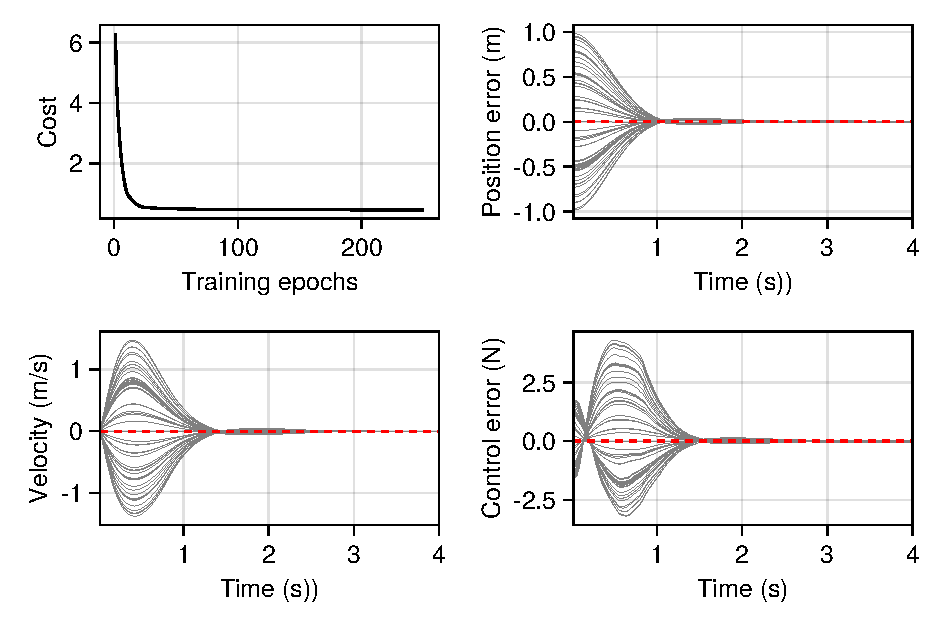
\includegraphics[width=0.47\textwidth]{Images/lbdn_rl.pdf}
    \caption{Loss curve and simulation results from the LBDN RL policy controlling the box system in Figure \ref{fig:rl-box}. The LBDN policy can push the box to any desired location in the domain of interest. The position and controller errors are $\Delta q$ and $\Delta u$ from Equation \ref{eqn:rl-costfunc}, respectively.}
    \label{fig:rl-results}
\end{figure}

% Using DiffLBDN
\subsubsection{Advantages of separate parameters and models} \label{sec:rl-comptime}

As discussed in Section \ref{sec:separate-params}, there is a trade-off between convenience and performance in \verb|RobustNeuralNetworks.jl|. The \verb|DiffLBDN| and \verb|DiffREN| wrappers exist to allow users to train robust models in a \verb|Flux.jl|-like manner. These wrappers convert a model parameterization to its explicit form each time they are called, hence the user does \textit{not} have to re-construct the model in the loss function.
\begin{lstlisting}[language = Julia]
loss2(model, x0, qref, uref) = 
    cost(rollout(model, x0, qref), qref, uref)
\end{lstlisting}

The cost is computation speed, particular in an RL context. Careful inspection of the \verb|rollout()| function shows that the \verb|model| is evaluated many times within the loss function before the learnable parameters are updated with \verb|Flux.update!()|. As discussed in the Section \ref{sec:separate-params}, the major computational bottleneck in training RENs and LBDNs is the conversion from learnable (direct) parameters to an explicit model. Constructing the model only when the parameters are updated therefore saves considerably on computation time, particularly for large models.

For example, suppose we train single-hidden-layer LBDNs with $n = 2, 2^2, \ldots, 2^9$ neurons over 100 epochs on our box RL problem, and log the time taken to train each model when using both \verb|LBDN| and \verb|DiffLBDN|.

\newpage
\begin{lstlisting}[language = Julia]
function lbdn_compute_times(n; epochs=100)

    # Build model params and a model
    lbdn_ps = DenseLBDNParams{T}(nu, [n], ny, γ)
    diff_lbdn = DiffLBDN(deepcopy(lbdn_ps))

    # Time with LBDN vs DiffLBDN (respectively)
    t_lbdn = @elapsed (
        train_box_ctrl!(lbdn_ps, loss; epochs))
    t_diff_lbdn = @elapsed (
        train_box_ctrl!(diff_lbdn, loss2; epochs))
    return [t_lbdn, t_diff_lbdn]

end

# Evaluate computation time
# Run it once first for just-in-time compiler
ns = 2 .^ (1:9)
lbdn_compute_times(2; epochs=1)
comp_times = reduce(hcat, lbdn_compute_times.(ns))
\end{lstlisting}

The results are plotted in Figure \ref{fig:rl-comptime}. Even for a single-layer LBDN with $2^9 = 512$ neurons, it is clear that using \verb|DiffLBDN| takes an order of magnitude longer to train than only constructing the \verb|LBDN| model each time the \verb|loss()| function is called. If we were training dynamic models with REN, the computational overhead of using \verb|DiffREN| instead of \verb|REN| would be even more extreme, since the conversion from direct to explicit parameters in a REN is typically more computationally expensive than for LBDNs. It is for this reason that we strongly recommend using the \verb|LBDN| and \verb|REN| wrappers if many evaluations of the model are required before \verb|Flux.update!()| (or equivalent) is called, as in RL.

\begin{figure}[ht]
    \centering
    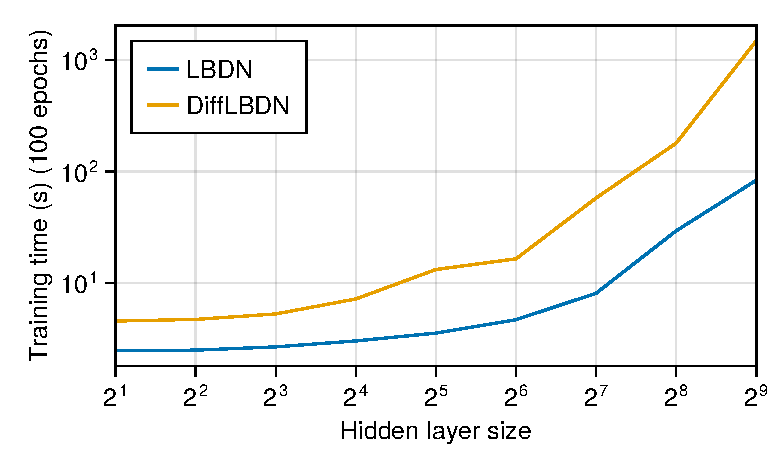
\includegraphics[width=0.47\textwidth]{Images/lbdn_rl_comptime.pdf}
    \caption{Training time as a function of hidden-layer size for a single-hidden-layer LBDN constructed with both the \texttt{LBDN} and \texttt{DiffLBDN} wrappers. Using the \texttt{LBDN} wrapper for RL is significantly more efficient than re-constructing the explicit model at every evaluation of the \texttt{DiffLBDN} model.}
    \label{fig:rl-comptime}
\end{figure}